%%%%%%%%%%%%%%%%%%%%%%%%%%%%%%%%%%%%%%%%%%%%%%%%%%%%%%%%%%%%%%%%%
% Contents: Theorie - Diplomarbeit, FH Regensburg               %
%                          11.03.2003                           %
%---------------------------------------------------------------%
%                          Theorie.tex                          %
%                      by Vorname Nachname                      %
%                         mail@mail.com                         %
%%%%%%%%%%%%%%%%%%%%%%%%%%%%%%%%%%%%%%%%%%%%%%%%%%%%%%%%%%%%%%%%%

\chapter{Theoretische Grundlagen}

blablabla

\section{Allgemeines und Historisches}

trallalla

\begin{itemize}
 \item Punkt 1
  \item Punkt 2
  \item Punkt 3
\end{itemize}


\section{So und so}

In Abbildung~\ref{pic_vpa1} ist folgendes zu sehen\ldots

\begin{figure}[!h]
\begin{center}
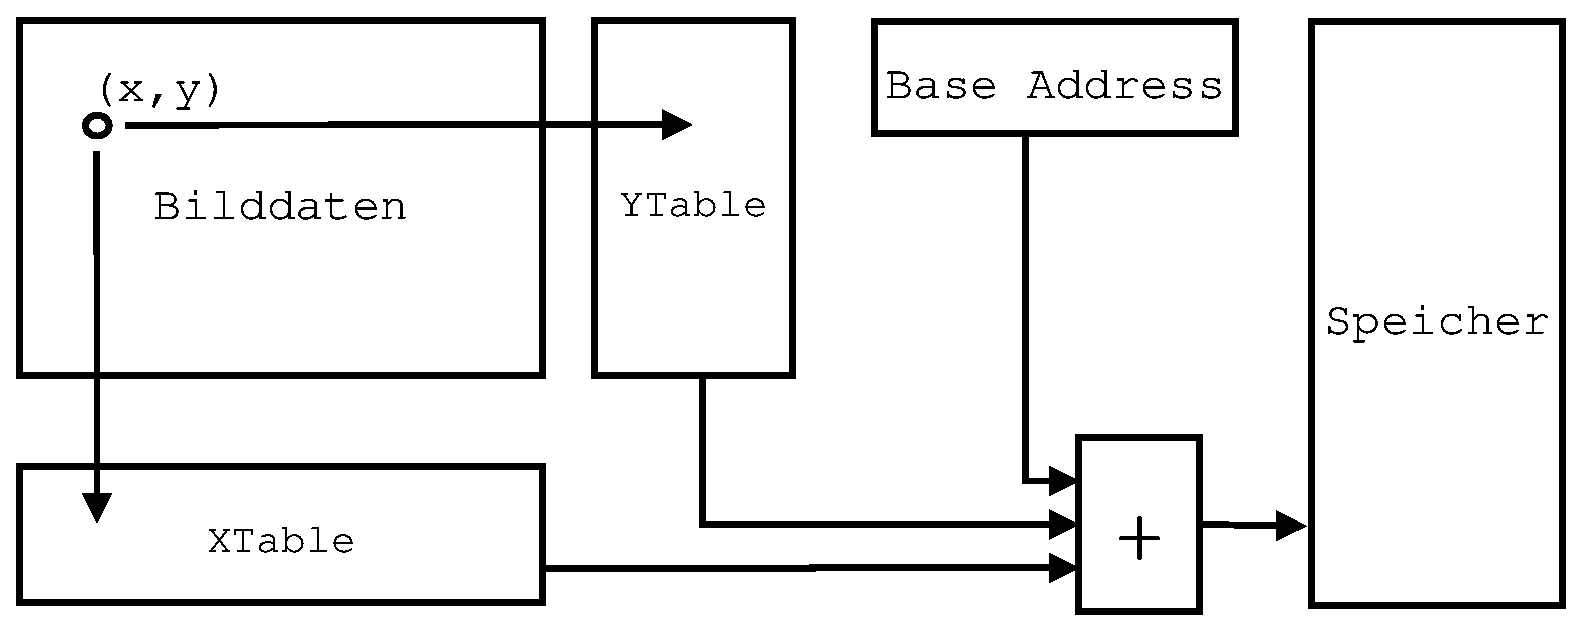
\includegraphics[width=0.9\textwidth]{images/vpa1.eps}
\caption{Pixeladressierung mit VPA} \label{pic_vpa1}
\end{center}
\end{figure}

In~\cite{zamperoni} steht dies und das\ldots

\subsection{Aufbau}
